\documentclass[11pt]{article}

% ---------------- Packages ----------------
\usepackage[margin=1in]{geometry}
\usepackage{amsmath,amssymb,amsthm}
\usepackage{graphicx}
\usepackage{hyperref}
\usepackage{fancyhdr}
\usepackage{enumitem}
\usepackage[UTF8]{ctex}
\usepackage{algorithm}
\usepackage{algpseudocode}
% ---------------- Header ----------------
\pagestyle{fancy}
\fancyhf{}
\lhead{Course Name}
\rhead{Homework \#1}
\cfoot{\thepage}

% ---------------- Title ----------------
\title{Homework 1}
\author{羊瑞 \\ 2300013091}
\date{\today}

% ---------------- Custom commands ----------------
\newcommand{\R}{\mathbb{R}}
\newcommand{\E}{\mathbb{E}}

% ---------------- Problem Environment ----------------
\newcounter{problem}

\newenvironment{problem}[1][]{
\stepcounter{problem}
\section*{Problem \theproblem\; #1}
}{}

\newenvironment{solution}{
\par\noindent\textbf{Solution.}\par\noindent
}{\qed}

\setlength{\parindent}{0pt}
% ---------------- Document ----------------
\begin{document}

\maketitle

\begin{problem} 
\begin{center}
    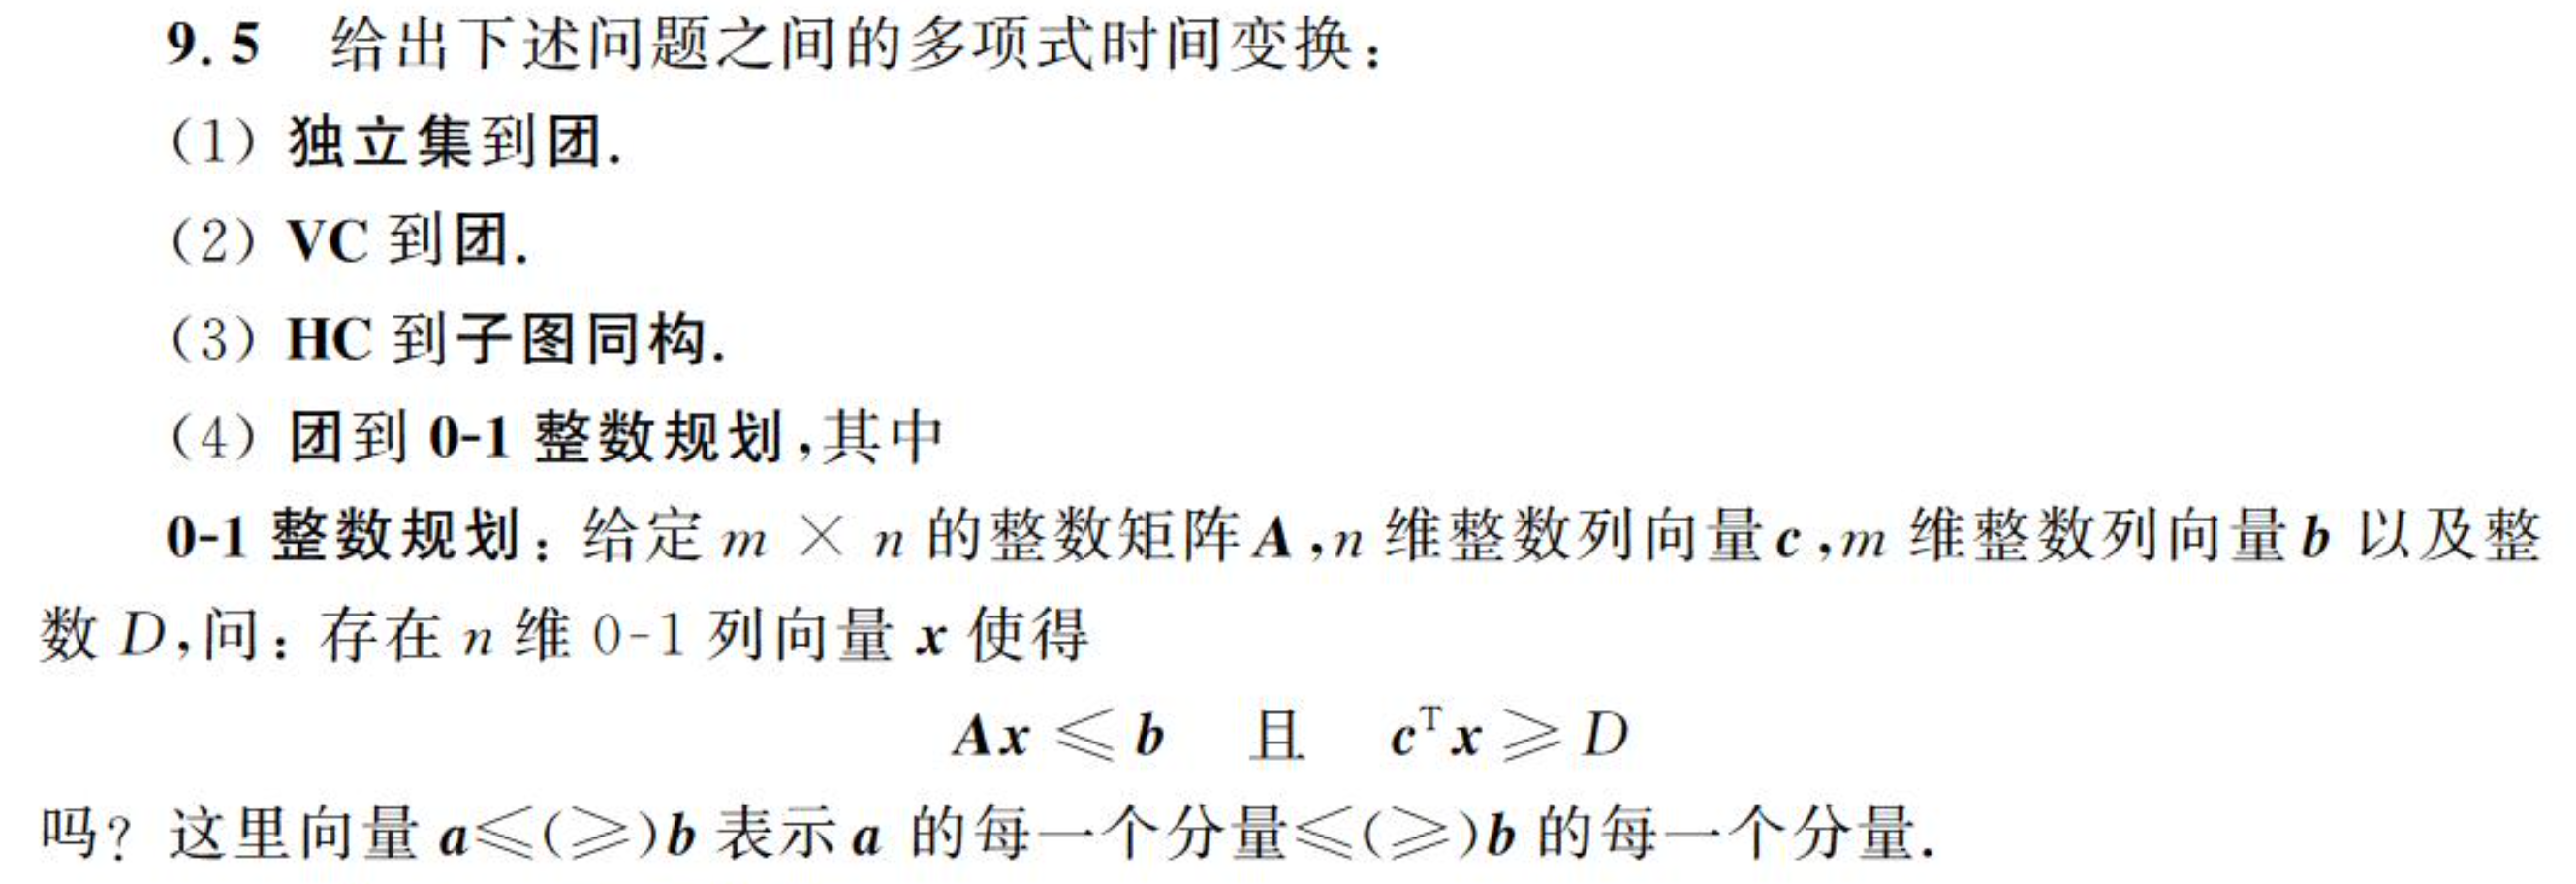
\includegraphics[width=0.6\textwidth]{problems/9.5.png}
\end{center}
\end{problem}

\begin{solution}
(1) 独立集到团

独立集问题的输入为
\[
(G,k),
\]
其中
\[
G=(V,E)
\]
是无向图，问题是判断 $G$ 中是否存在大小至少为 $k$ 的独立集。

构造 $G$ 的补图
\[
\overline{G}=(V,\overline{E}),
\]
其中
\[
(u,v)\in \overline{E}
\iff
u\neq v \text{ 且 } (u,v)\notin E.
\]

然后输出团问题实例
\[
(\overline{G},k).
\]

下面证明该变换正确。

若 $S\subseteq V$ 是 $G$ 中大小至少为 $k$ 的独立集，则对任意不同的
\[
u,v\in S,
\]
都有
\[
(u,v)\notin E.
\]
因此在补图中有
\[
(u,v)\in \overline{E}.
\]
所以 $S$ 是 $\overline{G}$ 中大小至少为 $k$ 的团。

反过来，若 $S$ 是 $\overline{G}$ 中大小至少为 $k$ 的团，则对任意不同的
\[
u,v\in S,
\]
都有
\[
(u,v)\in \overline{E}.
\]
根据补图定义可知
\[
(u,v)\notin E.
\]
因此 $S$ 是 $G$ 中大小至少为 $k$ 的独立集。

所以
\[
G \text{ 有大小至少为 } k \text{ 的独立集}
\iff
\overline{G} \text{ 有大小至少为 } k \text{ 的团}.
\]

构造补图只需要检查所有点对，因此时间复杂度为

\[
O(|V|^2).
\]

所以这是一个多项式时间变换。

(2)

顶点覆盖问题的输入为
\[
(G,k),
\]
其中
\[
G=(V,E),\qquad |V|=n.
\]
问题是判断 $G$ 中是否存在大小至多为 $k$ 的顶点覆盖。

构造 $G$ 的补图
\[
\overline{G}=(V,\overline{E}),
\]
然后输出团问题实例
\[
(\overline{G},n-k).
\]

下面证明该变换正确。

若 $C\subseteq V$ 是 $G$ 中大小至多为 $k$ 的顶点覆盖，则
\[
V-C
\]
中任意两个顶点之间在 $G$ 中都没有边。

否则，如果存在一条边
\[
(u,v)\in E
\]
且
\[
u,v\in V-C,
\]
那么这条边的两个端点都不在 $C$ 中，与 $C$ 是顶点覆盖矛盾。

因此
\[
V-C
\]
是 $G$ 中的独立集，并且

\[
|V-C|=n-|C|\geq n-k.
\]

由第 $(1)$ 问可知，$V-C$ 是 $\overline{G}$ 中大小至少为 $n-k$ 的团。

反过来，若 $\overline{G}$ 中存在大小至少为 $n-k$ 的团 $S$，则 $S$ 是 $G$ 中的独立集。令

\[
C=V-S.
\]

由于 $S$ 是独立集，所以 $G$ 中的每条边至少有一个端点不在 $S$ 中，即至少有一个端点在 $C$ 中。因此 $C$ 是 $G$ 的顶点覆盖。

并且

\[
|C|=n-|S|\leq k.
\]

所以

\[
G \text{ 有大小至多为 } k \text{ 的顶点覆盖}
\iff
\overline{G} \text{ 有大小至少为 } n-k \text{ 的团}.
\]

构造补图需要时间

\[
O(n^2),
\]

因此这是一个多项式时间变换。

(3)

哈密顿回路问题的输入为无向图

\[
G=(V,E),
\qquad |V|=n.
\]

问题是判断 $G$ 中是否存在一条经过每个顶点恰好一次的回路。

构造一个长度为 $n$ 的环图

\[
C_n=(V_H,E_H),
\]

其中

\[
V_H=\{u_1,u_2,\ldots,u_n\},
\]

\[
E_H=\{(u_1,u_2),(u_2,u_3),\ldots,(u_{n-1},u_n),(u_n,u_1)\}.
\]

然后构造子图同构问题实例

\[
(C_n,G).
\]

也就是说，问 $C_n$ 是否同构于 $G$ 的某个子图。

下面证明该变换正确。

若 $G$ 有哈密顿回路，则存在 $G$ 中 $n$ 个顶点的一个排列

\[
v_1,v_2,\ldots,v_n
\]

使得

\[
(v_1,v_2),(v_2,v_3),\ldots,(v_{n-1},v_n),(v_n,v_1)\in E.
\]

于是映射

\[
u_i\mapsto v_i,\qquad i=1,2,\ldots,n
\]

给出了从 $C_n$ 到 $G$ 的某个子图的同构。

因此 $C_n$ 同构于 $G$ 的一个子图。

反过来，若 $C_n$ 同构于 $G$ 的一个子图，则 $G$ 中存在 $n$ 个互不相同的顶点

\[
v_1,v_2,\ldots,v_n
\]

使得

\[
(v_1,v_2),(v_2,v_3),\ldots,(v_{n-1},v_n),(v_n,v_1)\in E.
\]

这正是一条经过 $G$ 中所有顶点恰好一次的回路，因此 $G$ 有哈密顿回路。

所以

\[
G \text{ 有哈密顿回路}
\iff
C_n \text{ 同构于 } G \text{ 的某个子图}.
\]

构造 $C_n$ 显然只需要

\[
O(n)
\]

时间，因此这是一个多项式时间变换。

(4)

团问题的输入为

\[
(G,k),
\]

其中

\[
G=(V,E),\qquad V=\{v_1,v_2,\ldots,v_n\}.
\]

问题是判断 $G$ 中是否存在大小至少为 $k$ 的团。

为每个顶点 $v_i$ 引入一个 $0$-$1$ 变量

\[
x_i\in\{0,1\}.
\]

含义为：

\[
x_i=
\begin{cases}
1, & \text{选择顶点 } v_i,\\
0, & \text{不选择顶点 } v_i.
\end{cases}
\]

为了保证被选择的顶点构成团，需要对于每一对非边

\[
(v_i,v_j)\notin E,\qquad i<j,
\]

加入约束

\[
x_i+x_j\leq 1.
\]

这表示两个不相邻的顶点不能同时被选中。

再令

\[
c=(1,1,\ldots,1)^T,
\qquad D=k.
\]

于是目标条件为

\[
c^Tx=\sum_{i=1}^n x_i\geq k.
\]

因此构造得到的 $0$-$1$ 整数规划为

\[
\begin{aligned}
&\text{是否存在 } x\in\{0,1\}^n,\\
&\text{使得 } x_i+x_j\leq 1,
\qquad \forall (v_i,v_j)\notin E,\ i<j,\\
&\text{且 } \sum_{i=1}^n x_i\geq k.
\end{aligned}
\]

把所有非边约束写成矩阵形式，即可得到

\[
Ax\leq b,
\qquad
c^Tx\geq D.
\]

下面证明该变换正确。

若 $G$ 中存在大小至少为 $k$ 的团 $S$，则令

\[
x_i=
\begin{cases}
1, & v_i\in S,\\
0, & v_i\notin S.
\end{cases}
\]

因为 $S$ 是团，所以任意两个被选中的顶点之间都有边。因此对于任意非边
\[
(v_i,v_j)\notin E,
\]
不可能同时有
\[
x_i=x_j=1.
\]
所以
\[
x_i+x_j\leq 1.
\]

并且

\[
\sum_{i=1}^n x_i=|S|\geq k.
\]

因此构造出的 $0$-$1$ 整数规划有可行解。

反过来，若该 $0$-$1$ 整数规划存在可行解 $x$，令

\[
S=\{v_i\mid x_i=1\}.
\]

由

\[
\sum_{i=1}^n x_i\geq k
\]

可知

\[
|S|\geq k.
\]

又因为对所有非边 $(v_i,v_j)\notin E$ 都有

\[
x_i+x_j\leq 1,
\]

所以 $S$ 中不可能同时包含两个不相邻的顶点。因此 $S$ 中任意两个不同顶点之间都有边，即 $S$ 是 $G$ 中的团。

所以

\[
G \text{ 有大小至少为 } k \text{ 的团}
\iff
\text{构造出的 } 0\text{-}1 \text{ 整数规划有可行解}.
\]

非边的数量至多为

\[
\binom{n}{2},
\]

因此构造矩阵 $A$、向量 $b$、向量 $c$ 和整数 $D$ 的时间为

\[
O(n^2).
\]

所以这是一个多项式时间变换。
\end{solution}

\begin{problem}
\begin{center}
    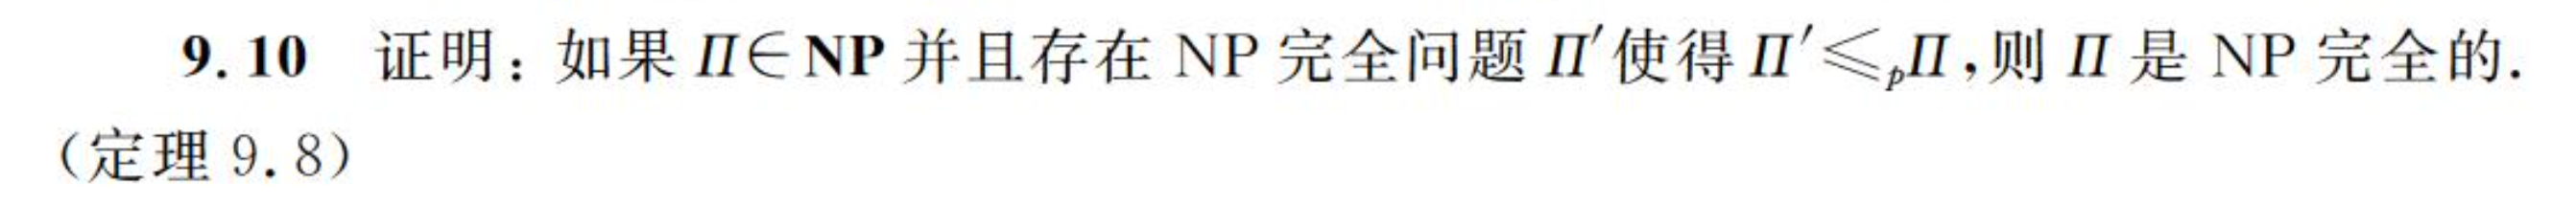
\includegraphics[width=0.6\textwidth]{problems/9.10.png}
\end{center}
\end{problem}

\begin{solution}
证明:

根据 NP 完全问题的定义，要证明 \(\Pi\) 是 NP 完全的，需要证明两点：

\[
(1)\quad \Pi\in \mathrm{NP};
\]

\[
(2)\quad \forall L\in \mathrm{NP},\ L\leq_p \Pi.
\]

题目已经给出

\[
\Pi\in \mathrm{NP}.
\]

因此只需证明任意 NP 中的问题都可以多项式时间归约到 \(\Pi\)。

由于 \(\Pi'\) 是 NP 完全问题，所以根据定义，对于任意

\[
L\in \mathrm{NP},
\]

都有

\[
L\leq_p \Pi'.
\]

又由题设可知

\[
\Pi'\leq_p \Pi.
\]

而多项式时间归约具有传递性，即若

\[
L\leq_p \Pi'
\quad\text{且}\quad
\Pi'\leq_p \Pi,
\]

则有

\[
L\leq_p \Pi.
\]

因此，对于任意

\[
L\in \mathrm{NP},
\]

都有

\[
L\leq_p \Pi.
\]

这说明 \(\Pi\) 是 NP-hard 的。

又因为题设已经给出

\[
\Pi\in \mathrm{NP},
\]

所以 \(\Pi\) 既属于 NP，又是 NP-hard 的。

因此

\[
\Pi \text{ 是 NP 完全的。}
\]

即

\[
\Pi \text{ is NP-complete}.
\]
\end{solution}

\begin{problem}
\begin{center}
    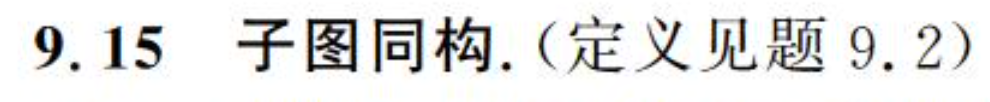
\includegraphics[width=0.6\textwidth]{problems/9.15.png}
\end{center}
\end{problem}

\begin{solution}
证明:

首先证明子图同构问题属于 NP。

给定一个映射
\[
f:V_1\to V_2,
\]
可以在多项式时间内验证：

\[
f \text{ 是否为单射，}
\]

并且对任意边
\[
(u,v)\in E_1,
\]
是否都有

\[
(f(u),f(v))\in E_2.
\]

若上述条件成立，则 \(G_1\) 同构于 \(G_2\) 的某个子图。因此子图同构问题的一个证书可以在多项式时间内验证，所以

\[
\text{子图同构}\in \mathrm{NP}.
\]

下面证明子图同构问题是 NP-hard 的。

由已知结论，哈密顿回路问题 \(HC\) 是 NP 完全的。我们将 \(HC\) 多项式时间归约到子图同构问题。

给定一个 \(HC\) 实例

\[
G=(V,E),
\qquad |V|=n.
\]

构造一个长度为 \(n\) 的环图

\[
C_n=(U,F),
\]

其中

\[
U=\{u_1,u_2,\ldots,u_n\},
\]

\[
F=\{(u_1,u_2),(u_2,u_3),\ldots,(u_{n-1},u_n),(u_n,u_1)\}.
\]

然后构造子图同构问题实例

\[
(C_n,G).
\]

也就是说，问 \(C_n\) 是否同构于 \(G\) 的某个子图。

下面证明该变换正确。

若 \(G\) 有哈密顿回路，则存在 \(G\) 中 \(n\) 个顶点的排列

\[
v_1,v_2,\ldots,v_n
\]

使得

\[
(v_1,v_2),(v_2,v_3),\ldots,(v_{n-1},v_n),(v_n,v_1)\in E.
\]

于是映射

\[
u_i\mapsto v_i,\qquad i=1,2,\ldots,n
\]

给出了 \(C_n\) 到 \(G\) 的某个子图的同构。因此

\[
C_n
\]

同构于 \(G\) 的一个子图。

反过来，若 \(C_n\) 同构于 \(G\) 的某个子图，则 \(G\) 中存在 \(n\) 个互不相同的顶点

\[
v_1,v_2,\ldots,v_n
\]

使得

\[
(v_1,v_2),(v_2,v_3),\ldots,(v_{n-1},v_n),(v_n,v_1)\in E.
\]

这正是一条经过 \(G\) 中每个顶点恰好一次的回路。因此 \(G\) 有哈密顿回路。

所以有

\[
G \text{ 有哈密顿回路}
\iff
C_n \text{ 同构于 } G \text{ 的某个子图}.
\]

构造 \(C_n\) 只需要

\[
O(n)
\]

时间，因此这是一个多项式时间归约：

\[
HC \leq_p \text{子图同构}.
\]

由于

\[
HC
\]

是 NP 完全问题，并且

\[
HC \leq_p \text{子图同构},
\]

所以子图同构问题是 NP-hard 的。

又因为已经证明

\[
\text{子图同构}\in \mathrm{NP},
\]

因此子图同构问题是 NP 完全的。

\[
\text{子图同构问题是 NP 完全的。}
\]
\end{solution}

\begin{problem}
\begin{center}
    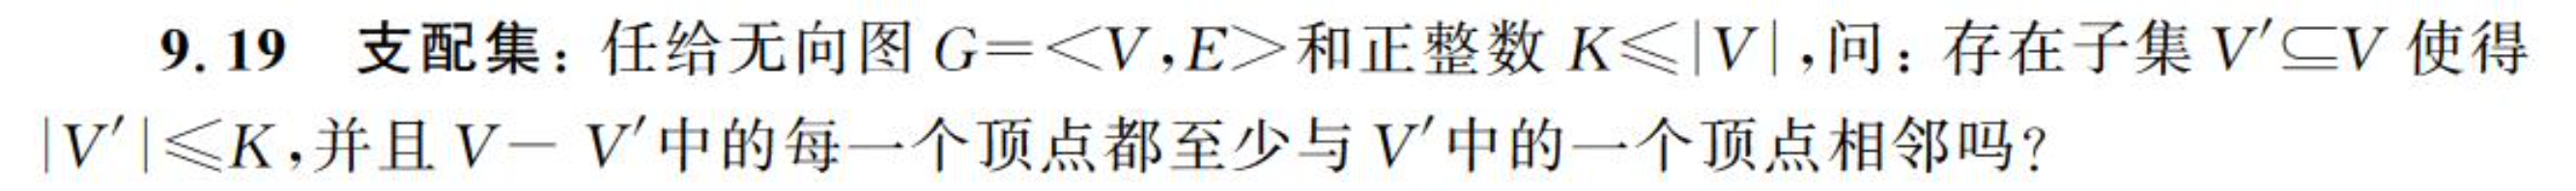
\includegraphics[width=0.6\textwidth]{problems/9.19.png}
\end{center}
\end{problem}

\begin{solution}
证明:

首先证明支配集问题属于 NP。

给定一个顶点子集 \(V'\)，可以在多项式时间内检查：

\[
|V'|\leq K,
\]

以及对每个

\[
v\in V-V',
\]

是否存在某个

\[
u\in V'
\]

使得

\[
(u,v)\in E.
\]

因此支配集问题的证书可以在多项式时间内验证，所以

\[
\text{支配集}\in \mathrm{NP}.
\]

下面证明支配集问题是 NP-hard 的。我们从顶点覆盖问题归约到支配集问题。

顶点覆盖问题的输入为

\[
G=(V,E),\qquad K,
\]

问是否存在

\[
C\subseteq V,\qquad |C|\leq K,
\]

使得 \(G\) 中每条边都至少有一个端点属于 \(C\)。

已知顶点覆盖问题是 NP 完全的。

对于顶点覆盖实例 \((G,K)\)，构造一个新的图

\[
G^\star=(V^\star,E^\star).
\]

构造如下：

\[
V^\star = V \cup \{x_e\mid e\in E\}.
\]

也就是说，对原图中的每条边

\[
e=(u,v)\in E,
\]

新建一个顶点 \(x_e\)。

边集 \(E^\star\) 按如下方式构造：

\[
\text{首先，将原来的顶点集合 } V \text{ 构造成一个团；}
\]

即对任意不同的

\[
u,v\in V,
\]

加入边

\[
(u,v).
\]

其次，对于每条边

\[
e=(u,v)\in E,
\]

加入两条边

\[
(x_e,u),\qquad (x_e,v).
\]

最后令

\[
K^\star=K.
\]

下面证明：

\[
G \text{ 有大小至多为 } K \text{ 的顶点覆盖}
\iff
G^\star \text{ 有大小至多为 } K^\star \text{ 的支配集}.
\]

\subsection*{充分性}

若 \(G\) 有大小至多为 \(K\) 的顶点覆盖 \(C\)，即

\[
C\subseteq V,\qquad |C|\leq K.
\]

我们证明 \(C\) 是 \(G^\star\) 的一个支配集。

首先，对于任意新加入的顶点 \(x_e\)，设

\[
e=(u,v).
\]

因为 \(C\) 是顶点覆盖，所以

\[
u\in C \quad \text{或} \quad v\in C.
\]

而在 \(G^\star\) 中，

\[
x_e
\]

与 \(u,v\) 都相邻，因此 \(x_e\) 被 \(C\) 支配。

其次，对于任意原顶点

\[
w\in V-C,
\]

由于 \(V\) 在 \(G^\star\) 中构成一个团，只要 \(C\neq \varnothing\)，则 \(w\) 与 \(C\) 中任意一个顶点相邻，因此 \(w\) 也被支配。

所以 \(C\) 是 \(G^\star\) 中大小至多为 \(K^\star\) 的支配集。

因此，

\[
G \text{ 有大小至多为 } K \text{ 的顶点覆盖}
\Rightarrow
G^\star \text{ 有大小至多为 } K^\star \text{ 的支配集}.
\]

\subsection*{必要性}

反过来，设 \(G^\star\) 有一个大小至多为 \(K^\star\) 的支配集 \(D\)，即

\[
D\subseteq V^\star,\qquad |D|\leq K.
\]

我们把 \(D\) 转化为原图 \(G\) 中的顶点集合 \(C\)。

若

\[
D
\]

中包含某个新顶点

\[
x_e,
\]

其中

\[
e=(u,v),
\]

则用 \(u\) 或 \(v\) 中任意一个端点替换 \(x_e\)。

经过这样的替换以后，得到一个只包含原图顶点的集合

\[
C\subseteq V,
\]

并且

\[
|C|\leq |D|\leq K.
\]

下面证明 \(C\) 是 \(G\) 的顶点覆盖。

任取原图中的一条边

\[
e=(u,v)\in E.
\]

在 \(G^\star\) 中存在对应的新顶点

\[
x_e.
\]

若

\[
x_e\in D,
\]

则在替换过程中，我们已经把 \(x_e\) 替换成了 \(u\) 或 \(v\) 中的一个，因此

\[
u\in C \quad \text{或} \quad v\in C.
\]

若

\[
x_e\notin D,
\]

由于 \(D\) 是支配集，所以 \(x_e\) 必须与 \(D\) 中某个顶点相邻。

而 \(x_e\) 在 \(G^\star\) 中只与 \(u\) 和 \(v\) 相邻，因此必有

\[
u\in D \quad \text{或} \quad v\in D.
\]

替换后仍有

\[
u\in C \quad \text{或} \quad v\in C.
\]

所以对于任意边

\[
e=(u,v)\in E,
\]

都有至少一个端点属于 \(C\)。因此 \(C\) 是 \(G\) 的顶点覆盖。

于是

\[
G^\star \text{ 有大小至多为 } K^\star \text{ 的支配集}
\Rightarrow
G \text{ 有大小至多为 } K \text{ 的顶点覆盖}.
\]

综上，

\[
G \text{ 有大小至多为 } K \text{ 的顶点覆盖}
\iff
G^\star \text{ 有大小至多为 } K^\star \text{ 的支配集}.
\]

该构造中，

\[
|V^\star|=|V|+|E|,
\]

并且构造原顶点团需要至多

\[
O(|V|^2)
\]

条边，连接新顶点与端点需要

\[
O(|E|)
\]

时间。因此整个变换可以在多项式时间内完成。

所以

\[
\text{顶点覆盖}\leq_p \text{支配集}.
\]

由于顶点覆盖问题是 NP 完全的，故支配集问题是 NP-hard 的。

又因为

\[
\text{支配集}\in \mathrm{NP},
\]

所以支配集问题是 NP 完全的。

\[
\boxed{\text{支配集问题是 NP 完全的。}}
\]
\end{solution}

\end{document}